%%%%%%%%%%%%%%%%%%%%%%%%%%%%%%%%%%%%%%%%%
% Arsclassica Article
% LaTeX Template
% Version 1.1 (10/6/14)
%
% This template has been downloaded from:
% http://www.LaTeXTemplates.com
%
% Original author:
% Lorenzo Pantieri (http://www.lorenzopantieri.net) with extensive modifications by:
% Vel (vel@latextemplates.com)
%
% Final modifications for this report by fedonman (fedonman.open-tech.gr)
%
% License:
% CC BY-NC-SA 3.0 (http://creativecommons.org/licenses/by-nc-sa/3.0/)
%
%%%%%%%%%%%%%%%%%%%%%%%%%%%%%%%%%%%%%%%%%

%----------------------------------------------------------------------------------------
%	PACKAGES AND OTHER DOCUMENT CONFIGURATIONS
%----------------------------------------------------------------------------------------

\documentclass[
12pt, % Main document font size
a4paper, % Paper type, use 'letterpaper' for US Letter paper
oneside, % One page layout (no page indentation)
%twoside, % Two page layout (page indentation for binding and different headers)
headinclude,footinclude, % Extra spacing for the header and footer
BCOR5mm, % Binding correction
]{article}

%%%%%%%%%%%%%%%%%%%%%%%%%%%%%%%%%%%%%%%%%
% Arsclassica Article
% Structure Specification File
%
% This file has been downloaded from:
% http://www.LaTeXTemplates.com
%
% Original author:
% Lorenzo Pantieri (http://www.lorenzopantieri.net) with extensive modifications by:
% Vel (vel@latextemplates.com)
%
% License:
% CC BY-NC-SA 3.0 (http://creativecommons.org/licenses/by-nc-sa/3.0/)
%
%%%%%%%%%%%%%%%%%%%%%%%%%%%%%%%%%%%%%%%%%

%----------------------------------------------------------------------------------------
%	REQUIRED PACKAGES
%----------------------------------------------------------------------------------------

\usepackage[
nochapters, % Turn off chapters since this is an article        
beramono, % Use the Bera Mono font for monospaced text (\texttt)
eulermath,% Use the Euler font for mathematics
pdfspacing, % Makes use of pdftex’ letter spacing capabilities via the microtype package
dottedtoc % Dotted lines leading to the page numbers in the table of contents
]{classicthesis} % The layout is based on the Classic Thesis style

\usepackage{arsclassica} % Modifies the Classic Thesis package

\usepackage[T1]{fontenc} % Use 8-bit encoding that has 256 glyphs

\usepackage[utf8]{inputenc} % Required for including letters with accents

\usepackage{graphicx} % Required for including images
\graphicspath{{Figures/}} % Set the default folder for images

\usepackage{enumitem} % Required for manipulating the whitespace between and within lists

\usepackage{lipsum} % Used for inserting dummy 'Lorem ipsum' text into the template

\usepackage{subfig} % Required for creating figures with multiple parts (subfigures)

\usepackage{amsmath,amssymb,amsthm} % For including math equations, theorems, symbols, etc

\usepackage{varioref} % More descriptive referencing

\usepackage{listings}

\usepackage{color}

%----------------------------------------------------------------------------------------
%	THEOREM STYLES
%---------------------------------------------------------------------------------------

\theoremstyle{definition} % Define theorem styles here based on the definition style (used for definitions and examples)
\newtheorem{definition}{Definition}

\theoremstyle{plain} % Define theorem styles here based on the plain style (used for theorems, lemmas, propositions)
\newtheorem{theorem}{Theorem}

\theoremstyle{remark} % Define theorem styles here based on the remark style (used for remarks and notes)

%----------------------------------------------------------------------------------------
%	HYPERLINKS
%---------------------------------------------------------------------------------------

\hypersetup{
%draft, % Uncomment to remove all links (useful for printing in black and white)
colorlinks=true, breaklinks=true, bookmarks=true,bookmarksnumbered,
urlcolor=webbrown, linkcolor=RoyalBlue, citecolor=webgreen, % Link colors
pdftitle={}, % PDF title
pdfauthor={\textcopyright}, % PDF Author
pdfsubject={}, % PDF Subject
pdfkeywords={}, % PDF Keywords
pdfcreator={pdfLaTeX}, % PDF Creator
pdfproducer={LaTeX with hyperref and ClassicThesis} % PDF producer
} % Include the structure.tex file which specified the document structure and layout

\hyphenation{Fortran hy-phen-ation} % Specify custom hyphenation points in words with dashes where you would like hyphenation to occur, or alternatively, don't put any dashes in a word to stop hyphenation altogether

\begin{document} % Document start

\pagenumbering{gobble} % Supress page numbering

%----------------------------------------------------------------------------------------
%	TITLE PAGE
%----------------------------------------------------------------------------------------

\begin{titlepage}

\newcommand{\HRule}{\rule{\linewidth}{0.5mm}} % Defines a new command for the horizontal lines, change thickness here

\center % Center everything on the page
 
%----------------------------------------------------------------------------------------
%	HEADING SECTIONS
%----------------------------------------------------------------------------------------

\textsc{\LARGE University of Peloponnese}\\[0.5cm] % Name of your university/college
\textsc{\Large National Observatory of Athens}\\[0.5cm] % Major heading such as course name
\textsc{\large MSc Space Science Technologies \& Applications}\\[1cm] % Minor heading such as course title

%----------------------------------------------------------------------------------------
%	TITLE SECTION
%----------------------------------------------------------------------------------------

\HRule \\[0.5cm]
{ \huge \bfseries Quality Control of daily GPS data from station KLOK}\\[0.2cm] % Title of your document
\HRule \\[1.5cm]
 
%----------------------------------------------------------------------------------------
%	AUTHOR SECTION
%----------------------------------------------------------------------------------------

\Large \emph{Authors}\\
Ioannis \textsc{Karavasilis}\\
Spiridon \textsc{Savvas}\\
Vyron \textsc{Vasileiadis}\\[3cm] % Your name

%----------------------------------------------------------------------------------------
%	DATE SECTION
%----------------------------------------------------------------------------------------

{\large \today}\\[3cm] % Date, change the \today to a set date if you want to be precise

%----------------------------------------------------------------------------------------
%	LOGO SECTION
%----------------------------------------------------------------------------------------

%\includegraphics{Logo}\\[1cm] % Include a department/university logo - this will require the graphicx package
 
%----------------------------------------------------------------------------------------

\vfill % Fill the rest of the page with whitespace

\end{titlepage}

%----------------------------------------------------------------------------------------
%	ABSTRACT & TABLE OF CONTENTS
%----------------------------------------------------------------------------------------

\begin{abstract}

NOA operates Klokotos GNSS station in Thessaly. In this report, we create an automated modular procedure of downloading Klokotos' data from the beginning of its operation until present day, performing quality control on the data and plotting the calculated values of the quality parameters (Multipath and SNR) over this period.

\end{abstract}

\newpage

\tableofcontents % Print the table of contents

\newpage 

\pagenumbering{arabic}

%----------------------------------------------------------------------------------------
%	HEADERS
%----------------------------------------------------------------------------------------

\renewcommand{\sectionmark}[1]{\markright{\spacedlowsmallcaps{#1}}} % The header for all pages (oneside) or for even pages (twoside)
%\renewcommand{\subsectionmark}[1]{\markright{\thesubsection~#1}} % Uncomment when using the twoside option - this modifies the header on odd pages
\lehead{\mbox{\llap{\small\thepage\kern1em\color{halfgray} \vline}\color{halfgray}\hspace{0.5em}\rightmark\hfil}} % The header style

\pagestyle{scrheadings} % Enable the headers specified in this block

%----------------------------------------------------------------------------------------
%	REPORT
%----------------------------------------------------------------------------------------

\section{Introduction}

NOA operates a National GNSS network of thirteen (13) stations transmitting real-time 1-s data to the control centre in Athens. One such station is station THL (Thessaly) is located at 39 deg. 33’ 53.065’’ North (latitude) and 22 deg. 00’ 51.7814’’ East (longitude). It is also known as Klokotos station, because of the nearby Klokotos village. It is equiped with both seismological and geodetical equipment.

The GNSS equipment was offered by INGV\footnote{http://www.ingv.it/} and installation was completed during May 2008. It comprises a Leica receiver (GRX 1200 Pro) with a choke-ring antenna (Leica AT 504). The sampling interval of observations is 1-s while a 5-Hz file is held on the ring-buffer with a life-time of 48 hrs. The 30-s data are available from the NOANET webpage\footnote{http://194.177.194.238:8080/noanetgsac} (code KLOK). An image of the installed equipment is shown in Figure~\ref{fig:klok}.

Every station is prone to errors, and to improve station's quality and further reduce common GPS errors, quality control is required. The most important quality parameters are Multipath in frequencies L1 and L2 (MP1 \& MP2) and SNR in both frequencies (SN1 \& SN2). Both can  be obtained  utilizing TEQC\footnote{https://www.unavco.org/software/data-processing/teqc/teqc.html}, which is a simple yet powerful toolkit to handle various GNSS data.

In this report, we create an automated procedure of downloading Klokotos' data from the beginning of its operation until present day, performing quality control on the data and plotting the calculated values of the quality parameters over this period.

\begin{figure}[h!]
\centering
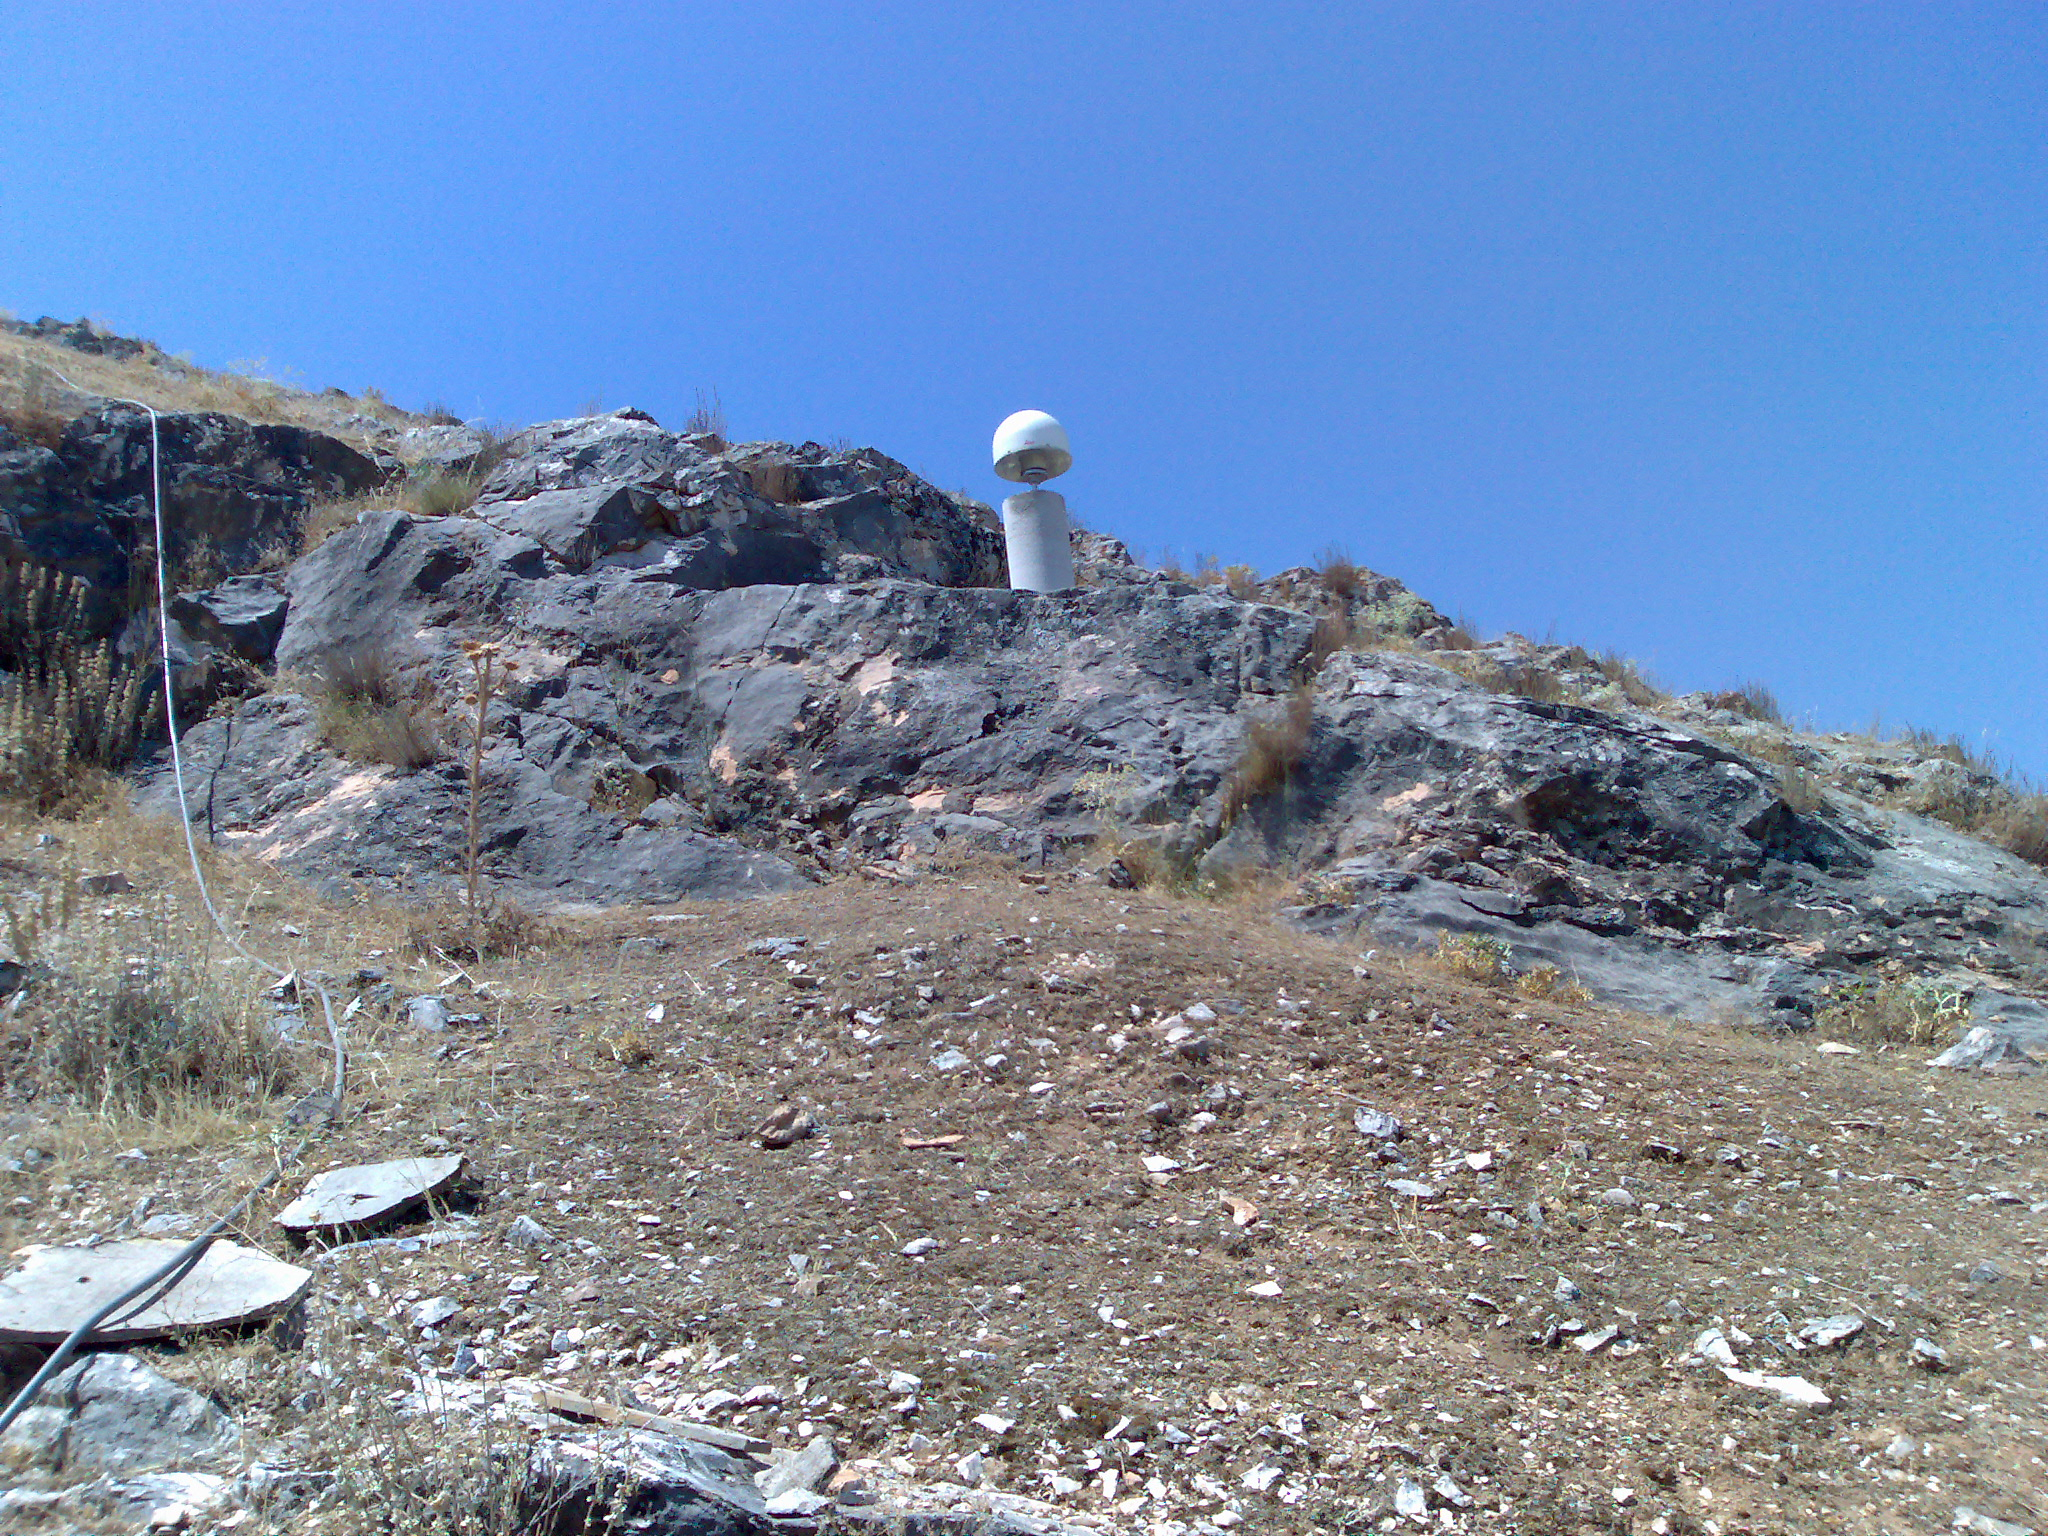
\includegraphics[scale=0.7]{klok.jpg}
\caption[text]{GNSS equipment of Klokotos station in Thessaly.}
\label{fig:klok}
\end{figure}


%----------------------------------------------------------------------------------------

\section{Methodology}

The procedure is stored in five different files, which are executed linearly. This approach, instead of a united file, offers modularization of the procedure and on-demand execution of the individual steps involved. For example, one could not download Klokotos' data if already has offline access to them, or could easily swap them with another station's data, while keeping the rest of the procedure intact.

\subsection{Download}
First step is to download the data from NOANET GSAC repository. Luckily, GSAC provides a search engine with many parameters. We are only concered about two; the file type and the site code. We check both \textit{RINEX GPS navigation file} and \textit{RINEX observation file} for downloading, while providing the code name \textit{KLOK} in the site code text field. These settings are shown in Figure~\ref{fig:gsac1}. GSAC provides a variety of different download options and formats, including a bash script containing \texttt{wget} commands. We choose this option as it can be easily included in our automated workflow. After clicking \texttt{'Wget Script for FTP download'} button we download \texttt{gsacwget.sh} and save it in our workspace directory.

\begin{figure}[h!]
\centering
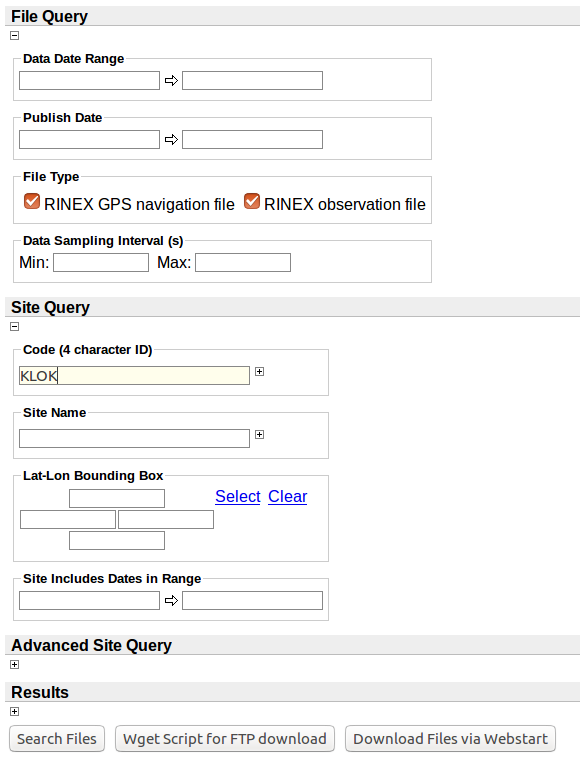
\includegraphics[scale=0.5]{gsac_1.png}
\caption[text]{Settings for downloading required Klokotos' data through NOANET GSAC repository}
\label{fig:gsac1}
\end{figure}

Next we execute \texttt{0\_download.sh} script. This script creates \texttt{zipped/} directory, if does not exist, and executes \texttt{gsacwget.sh} script in it. The result is the \texttt{zipped/} directory populated with lots of zipped \texttt{.Z} files, one for each day of observation.

\vfill

\vspace*{25pt}
\lstinputlisting[language=bash, basicstyle=\small\ttfamily, frame=bt, captionpos=b, title=\lstname]{0_download.sh}

\subsection{Unzip}
Next step is to unzip the files. For this task we execute \texttt{1\_unzip.sh} script. \texttt{1\_unzip.sh} creates the directory \texttt{unzipped/}, if it does not exists, extracts the contents of all the \texttt{.Z} archive files in \texttt{zipped/} directory and moves them to the \texttt{unzipped/} directory. This procedure's result is \texttt{unzipped/} directory populated with CompactRINEX observation files \texttt{*.*d} and RINEX GPS navigation files \texttt{*.*n}

\vspace*{25pt}
\lstinputlisting[language=bash, basicstyle=\small\ttfamily, frame=bt, captionpos=b, title=\lstname]{1_unzip.sh}

\subsection{Convert}

CompactRINEX observation files are not compatible with TEQC. We first need to convert them to regular RINEX observation files. For this task, we use \texttt{CRX2RNX} tool, which can be downloaded from its website\footnote{http://terras.gsi.go.jp/ja/crx2rnx.html}. To convert all files, we execute \texttt{2\_convert.sh}, which converts all CompactRINEX \texttt{*.*d} to RINEX \texttt{*.*o} files.

\vspace*{25pt}
\lstinputlisting[language=bash, basicstyle=\small\ttfamily, frame=bt, captionpos=b, title=\lstname]{2_convert.sh}

\subsection{Quality Control}
Next step is to perform the actual quality checking using TEQC. TEQC command for quality checking takes as input argument a single RINEX observation file, finds automatically the navigation file with the same name, and outputs a full report into a file with the same name and suffix \texttt{S}. For example, if we run \texttt{teqc +qc klok0010.10o} the report file would be  \texttt{klok0010.10S}. 

To  perform quality checking to all files we execute script \texttt{3\_qc.sh}, which also moves the report files to a seperate \texttt{reports/} directory to simplify the code of the last step.

\vspace*{25pt}
\lstinputlisting[language=bash, basicstyle=\small\ttfamily, frame=bt, captionpos=b, title=\lstname]{3_qc.sh}

\subsection{Analyse data \&  plot}
The final step involves analyzing the data from the produced reports and plotting the results. It is written in Python v3.6 and the source code can be examined in \texttt{4\_plot.py}.

\vspace*{25pt}
\lstinputlisting[language=Python, basicstyle=\small\ttfamily, frame=bt, captionpos=b, title=\lstname]{4_plot.py}
\vspace*{25pt}

Despite being larger than the rest scripts, \texttt{5\_plot.py} is essentialy simple. First, it reads all the filenames of the reports, stores them in a list and rearranges the list in chronological order. Then it  reads the  files  one by one, retrieves the quality parameters' values, multipath averages MP1 \& MP2 and mean SNRs SN1 \& SN2, and stores them in four lists keeping the chronological order. Finally, it create one plot with the the moving average timeseries and one plot with the two mean SNRs timeseries.


\section{Results}
Generated plots can be saved as image files and are shown in Figure~\ref{fig:results}. The first plot shows the distribution of multipath values over time, while the second shows the distribution of mean SNR values over time.

Studying the timeseries, it is clear that, while the range of values is minimal and predictable from the beginning of Klokotos operation in 2008, there has been a disturbance starting mid 2013 until mid 2015. This disturbance causes a large increase in multipath error for both frequencies L1 and L2. Also, there is a large decrease in SNR values for frequency L1 and a very minor decrease in SNR valuess for frequency L2.

We can assume that a large object was placed near the station during that period causing reflections of signals and thus multipath errors.

\begin{figure}[h!]
\centering
\hspace*{-3.5cm}
\begin{tabular}{cc}
\subfloat[Plot 1. Values of multipath averages over time.]{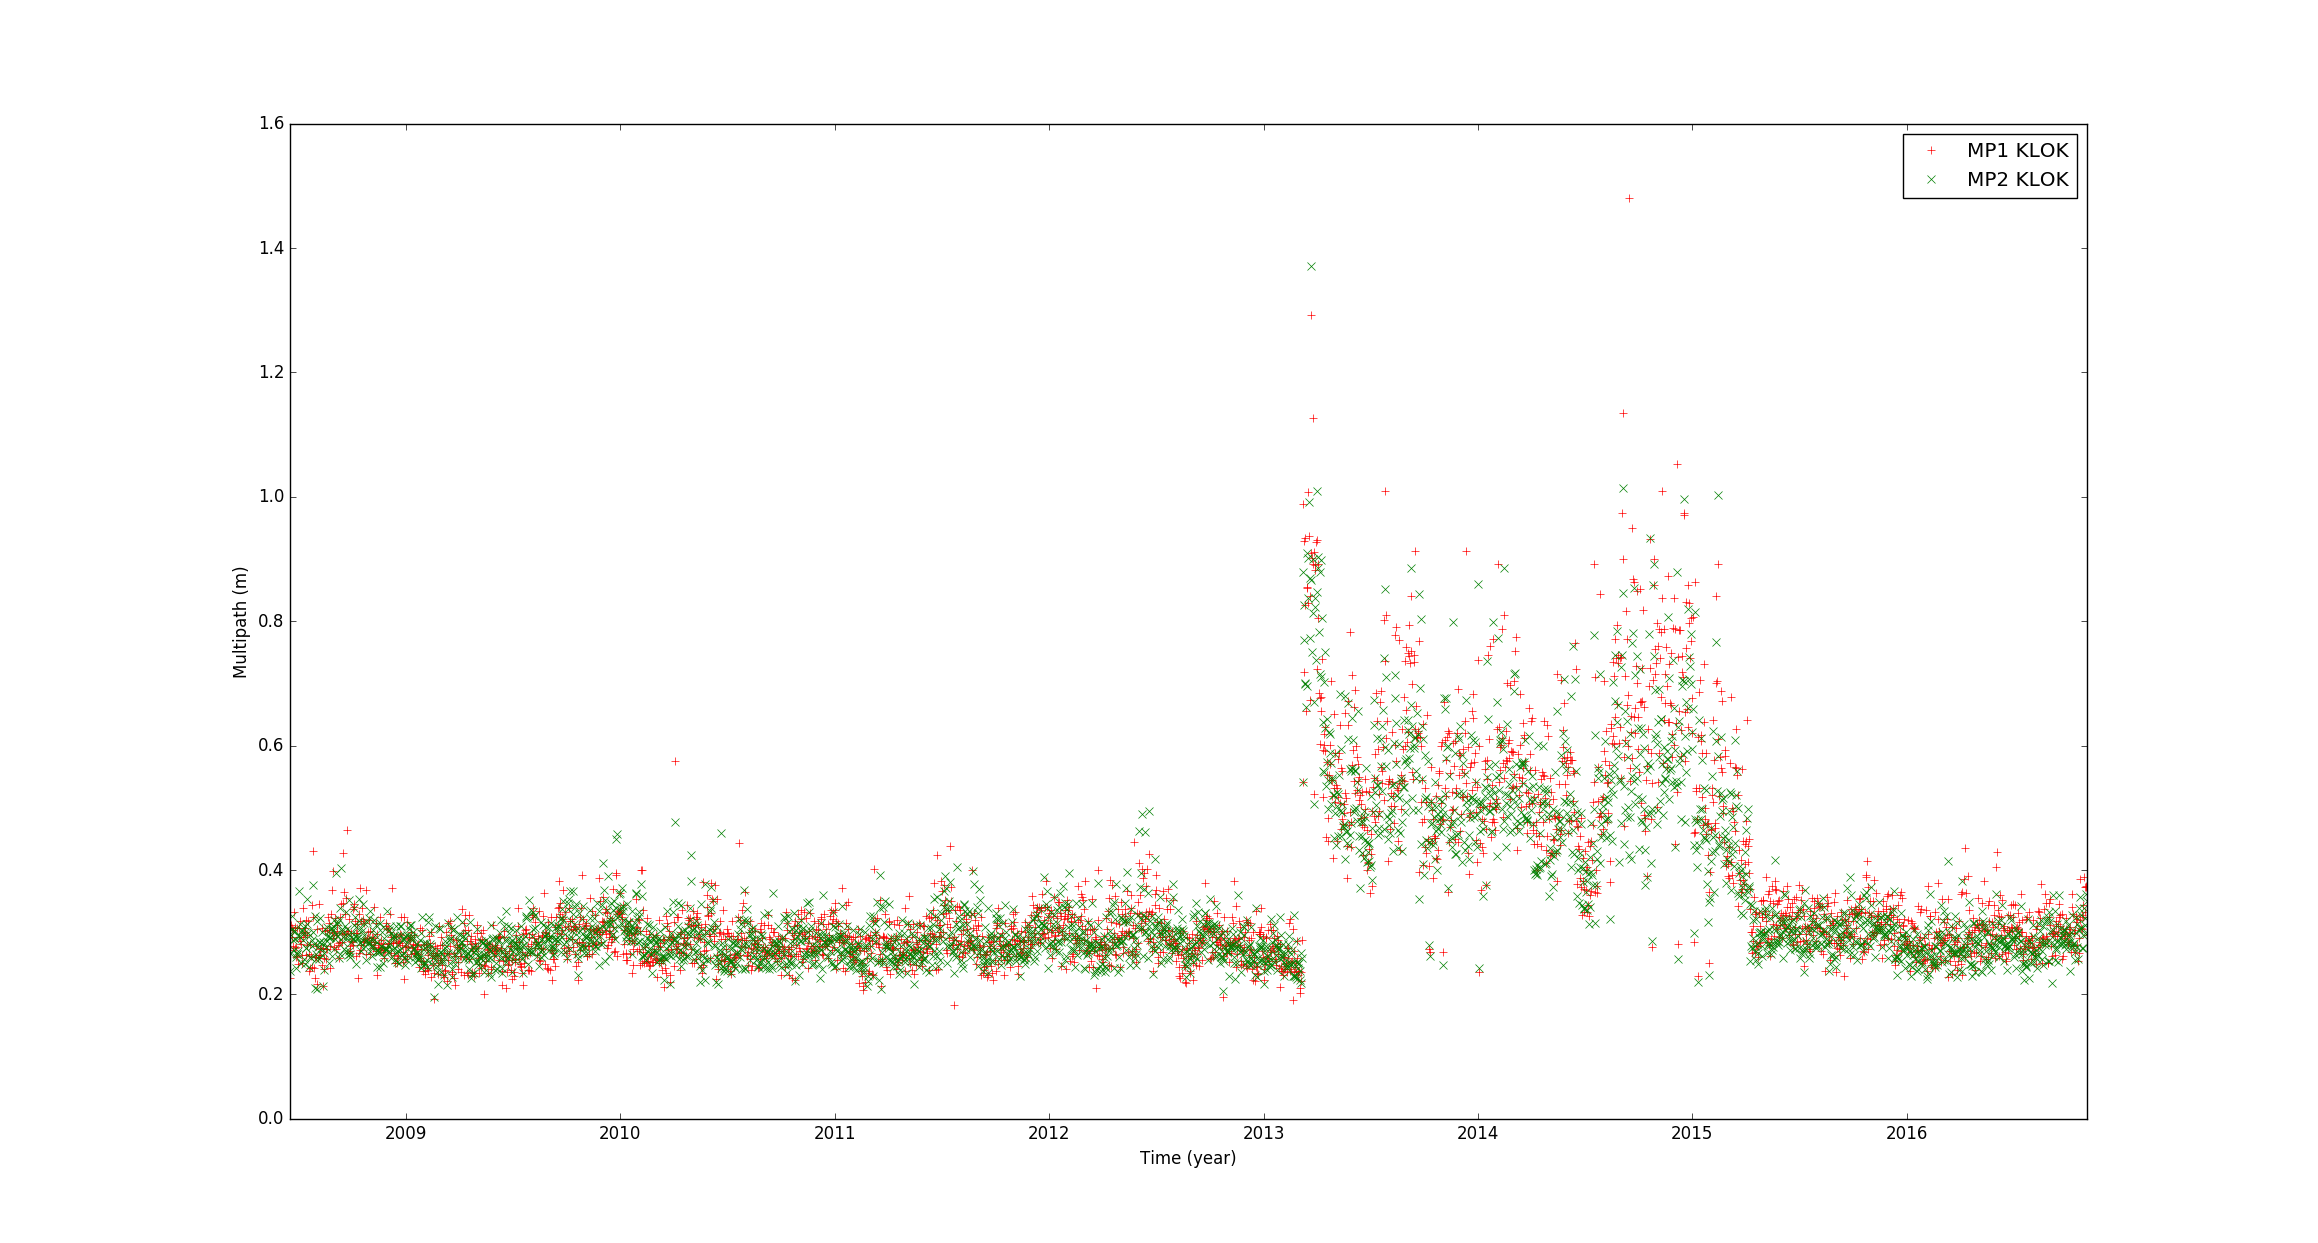
\includegraphics[scale=0.3]{figure_1.png}} \\
\subfloat[Plot 2. Values of mean SNRs over time.]{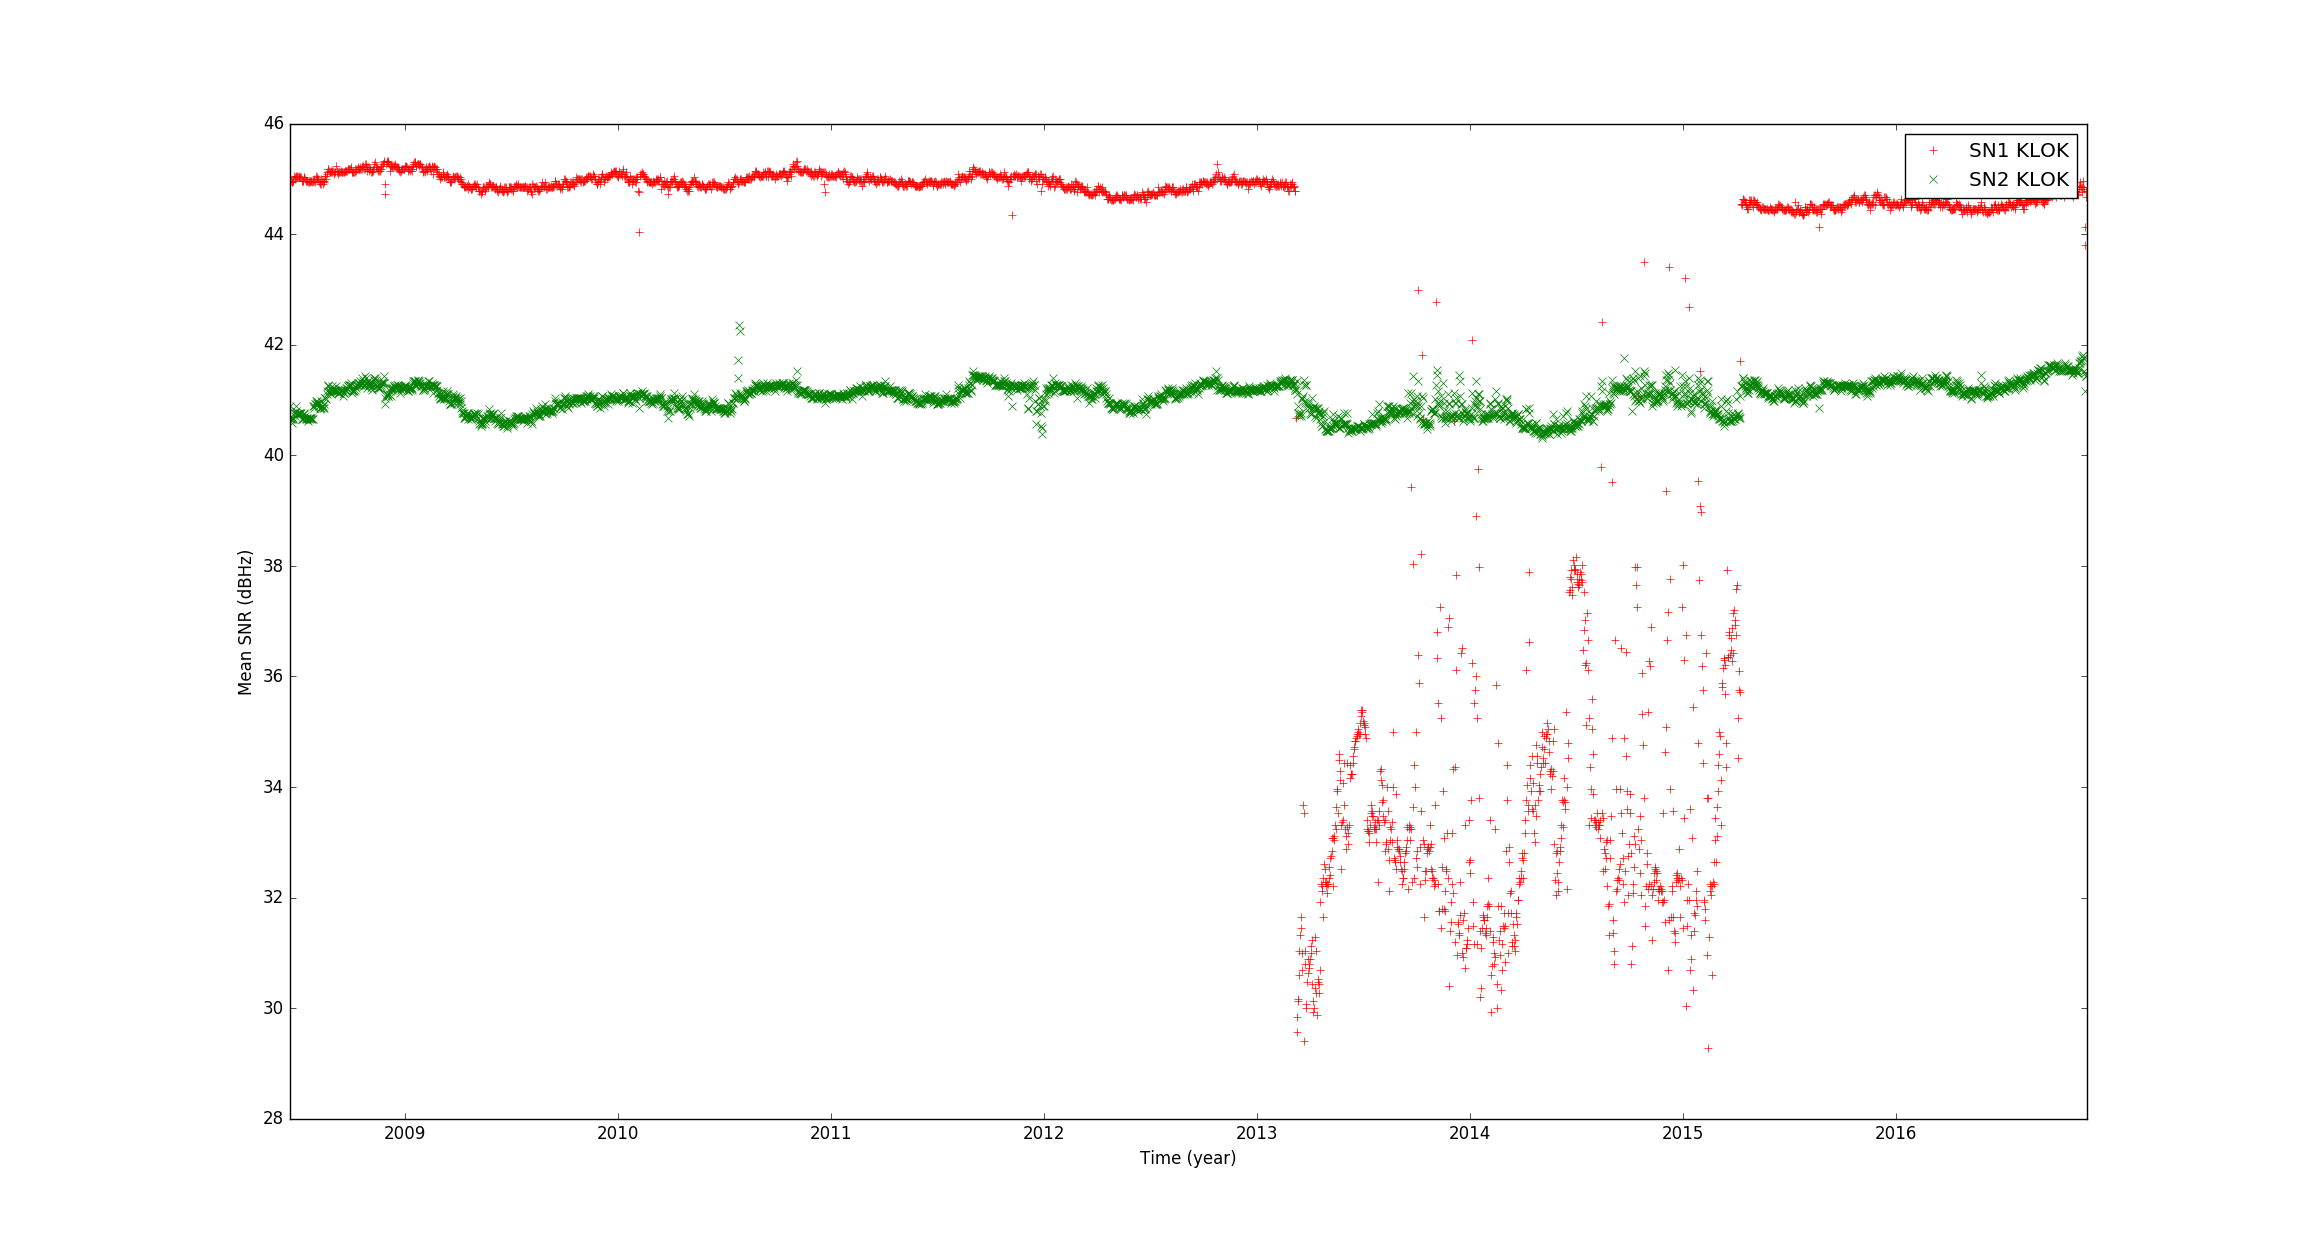
\includegraphics[scale=0.3]{figure_2snr.png}}
\end{tabular}
\caption{Results of quality control procedure}
\label{fig:results}
\end{figure}


%----------------------------------------------------------------------------------------
%	BIBLIOGRAPHY
%----------------------------------------------------------------------------------------

\renewcommand{\refname}{\spacedlowsmallcaps{References}} % For modifying the bibliography heading

\bibliographystyle{unsrt}

\bibliography{sample.bib} % The file containing the bibliography

%----------------------------------------------------------------------------------------

\end{document}